\section{Amanzi libraries}

This section describes Amanzi libraries, their limitations and possible 
ways to extend.

\subsection{WhetStone}
This is a low-level library that implements local matrices for various 
discretizations schemes. 
An abstract framework for 
Conceptual desing of a part of the library is presented in Fig.~\ref{fig:whetstone}.

Library {\it WhetStone} contains a factory of discretization scheme that could
be extended by including users schemes.
Example of such an extension is available.


\begin{figure}[h!]
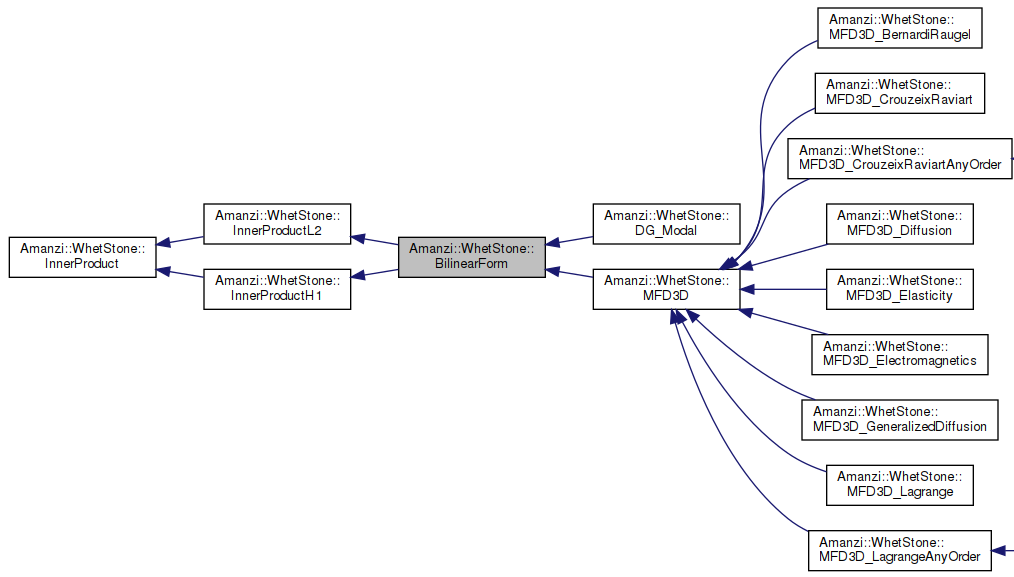
\includegraphics[width=1.0\textwidth]{figs/whetstone.png}
\caption{Partial dependency tree for library WhetStone.\label{fig:whetstone}}
\end{figure}

\subsection{Operators}

\begin{figure}[h!]
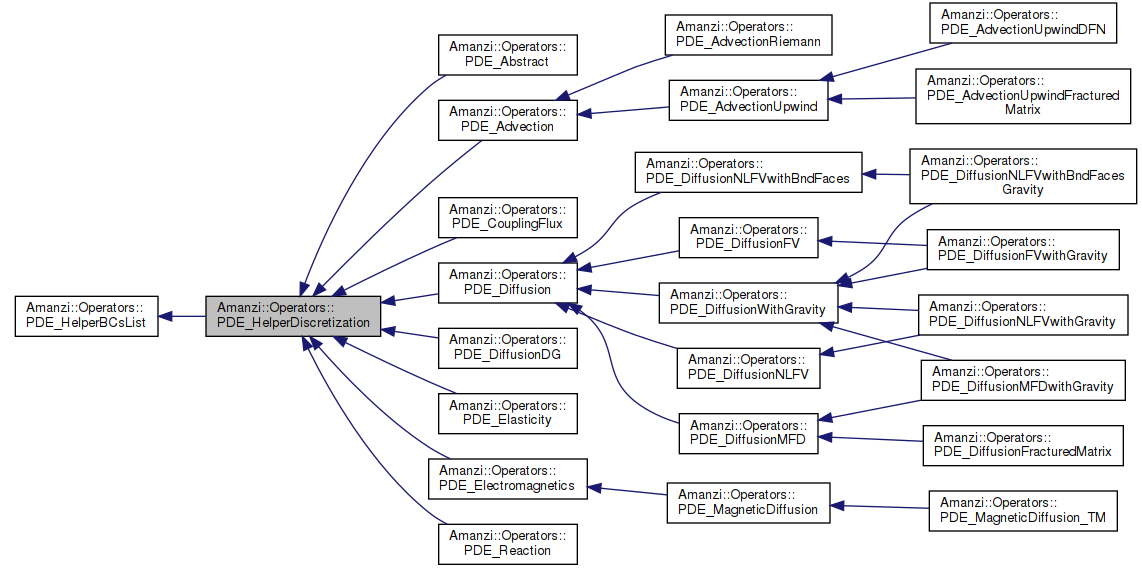
\includegraphics[width=1.0\textwidth]{figs/operators.png}
\caption{Partial dependency tree for library Operators.\label{fig:operators}}
\end{figure}


\subsection{PKs}

Bla-bla-bla

